\section{Double Thresholding}
\label{sec:double-thresholding}

Following non-maximum suppression, the edge pixels provide a clearer representation of true edges in the image. Nonetheless, some edge pixels might still appear due to noise and color differences. To eliminate these false positives, it is essential to discard edge pixels with low gradient values while retaining those with high gradient values.

This is achieved through a process called \emph{double thresholding}.

The Canny edge detector uses double thresholding to classify edge pixels into three categories: strong edges, weak edges, and non-edge pixels. The process is as follows:

\begin{enumerate}
    \item \textbf{Strong Edges:} Pixels with gradient magnitudes higher than a high threshold are classified as strong edges.
    \item \textbf{Non-Edge Pixels:} Pixels with gradient magnitudes lower than a low threshold are classified as non-edge pixels.
    \item \textbf{Weak Edges:} Pixels with gradient magnitudes between the high and low thresholds are classified as weak edges.
\end{enumerate}

The high and low thresholds are determined based on the gradient magnitude distribution in the image. Typically, the high threshold is set to a value that retains only strong edges, while the low threshold is set to a fraction of the high threshold.

In my version of implementation, I used ratios for the threshold --- $ T_{\text{high}} $ and $ T_{\text{high}} $ --- to determine the high and low thresholds. The ratios are provided as input parameters to the function. Then the high and low thresholds are calculated as follows:

\begin{align*}
    T_{\text{high}} & = r_{\text{max}} \cdot r_{\text{high\_ratio}} \\
    T_{\text{low}}  & = T_{\text{high}} \cdot r_{\text{low\_ratio}}
\end{align*}

The \emph{strong pixels} are assigned a value of 255, the \emph{weak pixels} are assigned a value lower than 255 (e.g., 100), and the \emph{non-edge pixels} are assigned a value of 0.

The images before and after double thresholding are shown in \autoref{fig:double-thresholding}.

\begin{figure}[ht]
    \centering
    \begin{subfigure}[b]{0.4\textwidth}
        \centering
        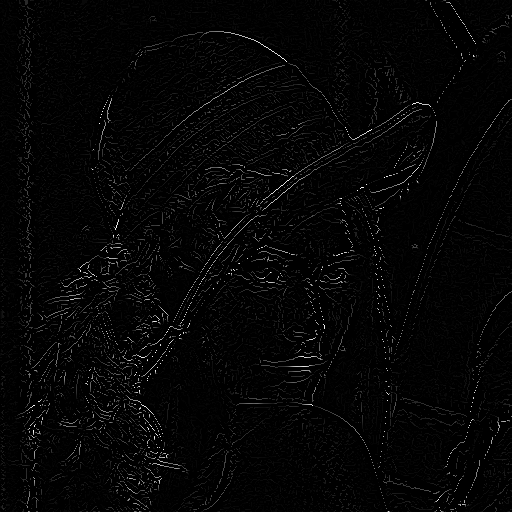
\includegraphics[width=0.9\textwidth]{lenna_6_non_max_suppressed.png}
        \caption{After Non-Maximum Suppression}
    \end{subfigure}
    \hfill
    \begin{subfigure}[b]{0.4\textwidth}
        \centering
        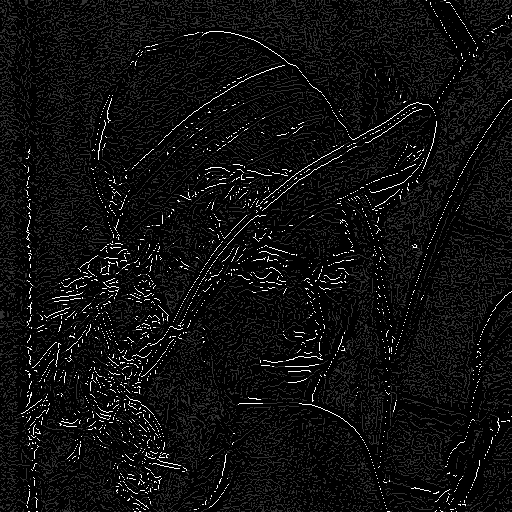
\includegraphics[width=0.9\textwidth]{lenna_7_double_thresholded.png}
        \caption{After Double Thresholding}
    \end{subfigure}
    \caption{Effect of Double Thresholding}
    \label{fig:double-thresholding}
\end{figure}